\documentclass[11pt,a4paper]{article}

% ---------- arxiv-style preamble ----------
\usepackage[margin=1in]{geometry}
\usepackage{amsmath,amssymb,amsthm}
\usepackage{graphicx}
\usepackage{longtable}
\usepackage{booktabs}
\usepackage{siunitx}
\usepackage{hyperref}
\usepackage{xcolor}
\usepackage[numbers,sort&compress]{natbib}
\usepackage{tikz}
\usetikzlibrary{positioning,arrows.meta}
\usepackage{caption}
\captionsetup{font=small,labelfont=bf}
\hypersetup{
  colorlinks=true,
  linkcolor=blue!50!black,
  citecolor=blue!50!black,
  urlcolor=blue!50!black
}

\newcommand{\sig}{\sigma}
\newcommand{\Dn}{D(n)}
\newcommand{\tierF}{\textcolor{blue!60!black}{$\blacklozenge$}\,\textsc{formal}}
\newcommand{\tierN}{\textcolor{green!45!black}{$\blacksquare$}\,\textsc{numerical}}
\newcommand{\tierR}{\textcolor{red!70!black}{$\bigtriangledown$}\,\textsc{falsified}}
\newcommand{\tierC}{\textcolor{orange!85!black}{$\circ$}\,\textsc{citation}}

\theoremstyle{definition}
\newtheorem{claim}{Claim}
\newtheorem{falsifier}{Pre-registered falsifier}

\title{
  \textbf{The \texorpdfstring{$n=6$}{n=6} Exclusivity Atlas}\\[4pt]
  \large A verify-driven closed-negative cluster: how machine-checked
  falsification tightens the \texorpdfstring{$\{1,6\}$}{\{1,6\}} arithmetic-function
  locus from an identity to an exclusive, non-lifting, scale-stable phenomenon
}

\author{
  TECS-L domain (NOVEL axis, F family), \texttt{hexa-lang}\\
  \normalsize\textit{dancinlab}\\[2pt]
  \normalsize\href{https://github.com/dancinlab/hexa-lang}{\texttt{github.com/dancinlab/hexa-lang}}
}

\date{\today}

\begin{document}

\maketitle

% =========================================================================
\begin{abstract}
The first perfect number $6$ sits at the centre of a small cluster of
arithmetic-function identities --- most prominently
$\sig(n)\phi(n)=n\tau(n)$, which a closed-form theorem (the TECS-L atlas atom
\textsf{M10}) proves holds for \emph{exactly} $n\in\{1,6\}$ over all positive
integers. A natural follow-up question is not whether the identities hold ---
that is settled --- but whether the \emph{specialness} of $\{1,6\}$ is an
isolated coincidence or whether it propagates: to amicable / quasi-perfect /
multiply-perfect neighbours, to perfect-number siblings such as $28$, to large
or structurally notable arguments, and upward to the modular-curve tower
$\Gamma_0(N)\to\Gamma_1(N)\to X(N)$. This paper aggregates the
\emph{NOVEL axis} of the TECS-L verification campaign --- the lane that hunts
\emph{outside} the known, as opposed to the lanes that re-ground known
identities --- and shows that it operates as a \textbf{verify-driven
exclusivity engine}. Rather than only confirming $n=6$ identities, it
systematically \emph{rules out} the adjacent space: we pre-register and then
machine-check (under the \texttt{hexa verify} tier rubric,
\textsection\ref{sec:method}) a battery of plausible ``$n=6$-like''
generalisations and find them all \emph{deterministically false}. Concretely we
report (i) seven exact-integer closed-negatives from the closed-negative miner
(\textsf{F5}); (ii) a non-lift result showing $\sig\phi=n\tau\Leftrightarrow\{1,6\}$
is a $\Gamma_0$-level phenomenon that does \emph{not} survive ascent to
$\Gamma_1(N)/X(N)$, whose index is smooth in $N$ (\textsf{F7}); and (iii) a
scale-extension sweep confirming $\Dn:=\sig(n)\phi(n)-n\tau(n)\neq0$ at seven
notable arguments up to $n=33550336$, extending the original $[1,100]$ sweep by
a factor of $\sim\!3.4\times10^{5}$ (\textsf{F6}). Counting both the F5
falsifiers and the F6/F7 negatives, the cluster comprises
\emph{ten or more deterministic closed-negatives}. The headline is the
\emph{cluster itself}: $\{1,6\}$ is not merely the support of an identity but an
\emph{exclusive}, \emph{non-lifting}, and \emph{scale-stable} arithmetic
locus. Every negative is a pre-registered falsifier resolved by exact integer
arithmetic --- no tolerance, no probabilistic claim --- which satisfies the
\textsf{paper\_significance} and \textsf{paper\_negative\_ok} gates of the host
project's discovery governance.
\end{abstract}

\tableofcontents

% =========================================================================
\section{Statement: the exclusivity thesis and its falsifiers}
\label{sec:statement}

\subsection{Background: the positive kernel}

Let $\sig$, $\phi$, $\tau$, $\mu$ denote the classical arithmetic functions
(sum of divisors, Euler totient, number of divisors, M\"obius function). The
positive kernel of this paper is a single theorem, already proved and folded
into the TECS-L theorem atlas as atom \textsf{M10}
(\textsf{tecs\_l\_up\_theorem}):

\begin{claim}[M10, the positive kernel]\label{cl:m10}
For all positive integers $n$,
\[
  \sig(n)\,\phi(n) = n\,\tau(n)
  \qquad\Longleftrightarrow\qquad
  n\in\{1,6\}.
\]
Equivalently, with the discrepancy $\Dn:=\sig(n)\phi(n)-n\tau(n)$, we have
$\Dn=0\Leftrightarrow n\in\{1,6\}$ and $\Dn\neq0$ otherwise.
\end{claim}

Claim~\ref{cl:m10} is a closed-form result; it is not the subject under test
here. What \emph{is} under test is the surrounding folklore: $6$ is the first
perfect number, the smallest squarefree even number, the order of the smallest
non-abelian group, and so on, and a large number of ``$6$ is special''
statements circulate without it being made precise \emph{which} ones encode the
$\{1,6\}$ exclusivity of Claim~\ref{cl:m10} and which are accidents that fail at
the very next candidate. The contribution of this paper is to draw that
boundary sharply, and to do so by \emph{falsification under verification}.

\subsection{The exclusivity thesis}

\begin{claim}[Exclusivity thesis]\label{cl:thesis}
The locus $\{1,6\}$ of Claim~\ref{cl:m10} is not an isolated identity but an
\emph{exclusive, non-lifting, scale-stable} arithmetic phenomenon:
\begin{enumerate}
\item[\textbf{(E)}] \emph{Exclusive.} Each of the obvious ``$n=6$-like''
  generalisations --- amicable membership as an aliquot fixed point,
  quasi-perfection $\sig(n)=2n+1$, multiply-perfect abundancy transfer, the
  sibling identity $n\phi(n)=\sig(n)$ off $\{1,6\}$, M\"obius $6$-periodicity,
  and the perfect $\Rightarrow$ superperfect implication --- is
  \emph{deterministically false}. The locus admits no loosening to a
  neighbouring conjecture.
\item[\textbf{(N)}] \emph{Non-lifting.} The $\{1,6\}$ distinction is a
  $\Gamma_0$-level (arithmetic-function) phenomenon. It does \emph{not} lift to
  the modular-curve tower $\Gamma_1(N)/X(N)$, whose index is a smooth
  multiplicative function of $N$ with no peak or collapse at $N=6$.
\item[\textbf{(S)}] \emph{Scale-stable.} The discrepancy $\Dn\neq0$ persists at
  every notable large argument tested --- primorials, factorials, pure powers
  of two, and the fourth and fifth perfect numbers --- up to
  $n=33550336$.
\end{enumerate}
\end{claim}

The three components are tested by three pre-registered falsifier batteries,
sourced respectively from the F5, F7, and F6 lanes of the TECS-L NOVEL axis.
We state them here as falsifiers (a result that, had it come out the other
way, would have refuted the corresponding component of the thesis), in keeping
with the host project's \textsf{paper\_significance} requirement of a
pre-registered falsifier plus a real measurement.

\begin{falsifier}[component E, from F5]\label{f:E}
There exists a positive integer witnessing one of the six ``$n=6$-like''
generalisations CN1--CN6 of \textsection\ref{sec:verif-f5}. A single such
witness, computed exactly, would show the locus is \emph{not} exclusive and
falsify component~(E).
\end{falsifier}

\begin{falsifier}[component N, from F7]\label{f:N}
The modular-curve index $[\mathrm{SL}_2(\mathbb{Z}):\Gamma_1(N)]$ or
$[\mathrm{SL}_2(\mathbb{Z}):X(N)]$ exhibits a $\{1,6\}$-type distinction
(a peak, singularity, or arithmetic-function collapse) at $N=6$ that is absent
at neighbouring $N$. Such a distinction would show the $\{1,6\}$ specialness
lifts up the tower and falsify component~(N).
\end{falsifier}

\begin{falsifier}[component S, from F6]\label{f:S}
There exists a notable large argument $n\notin\{1,6\}$ (primorial, factorial,
power of two, or perfect number) with $\Dn=0$. A single such argument would
show the identity recurs at scale and falsify component~(S).
\end{falsifier}

The remainder of the paper resolves all three falsifiers deterministically in
the negative, which is precisely the affirmation of Claim~\ref{cl:thesis}: the
falsifiers are designed so that their \emph{failure to fire} \emph{is} the
finding.

% =========================================================================
\section{Method: closed-negative mining under \texttt{hexa verify}}
\label{sec:method}

\subsection{The verification discipline and tier rubric}

Every numerical statement in this paper is settled by \texttt{hexa verify}, the
host language's verification gate, in its \texttt{-{}-expr} form
\[
  \texttt{hexa verify -{}-expr <fn> <n> <v>}
\]
which recomputes the hexa-native closed form of arithmetic function
\texttt{<fn>} at argument \texttt{<n>}, compares it to the expected value
\texttt{<v>} by \emph{exact integer arithmetic}, and emits a verdict tier. The
functions exercised here ($\sig$, $\phi$, $\tau$, $\mu$, \texttt{aliquot},
\texttt{is\_perfect}, \texttt{gamma0\_index}) are all live in the HEAD driver
(build \#1153). The relevant tiers are:

\begin{itemize}
\item \tierF: \textsc{supported-formal} --- the hexa-native closed form
  reproduces the expected value exactly (\texttt{calc == expected}). This is the
  tier of a confirmed component.
\item \tierN: \textsc{supported-numerical} --- a derived quantity (e.g. the
  product $\sig(n)\phi(n)$ or the discrepancy $\Dn$) computed by exact integer
  arithmetic on \tierF\ components.
\item \tierR: \textsc{falsified} --- \texttt{calc != expected}; the statement
  is deterministically false. This is the tier of a fired falsifier, and the
  payload of a closed-negative.
\item \tierC: \textsc{supported-by-citation} --- a quantity assembled from a
  cited closed-form formula on top of \tierF\ components (used for the modular
  index assembly in \textsection\ref{sec:verif-f7}).
\end{itemize}

A \emph{closed-negative} is a statement deliberately constructed to be
plausible (an apparent generalisation of an $n=6$ identity) and then shown to be
\tierR\ by exact recomputation. Crucially, each closed-negative is paired with
the \tierF\ truth-component it contradicts, so that the negative is anchored: we
exhibit both the wrong expected value and the right computed value side by side.
There is no tolerance, no floating point, and no probabilistic inference
anywhere in the battery (see \textsection\ref{sec:caveats}).

\subsection{The three mining lanes}

\paragraph{F5 --- closed-negative miner (component E).}
We enumerate six families of ``$n=6$-like'' conjectures (CN1--CN6, with CN4
split into CN4/CN4b), each obtained by taking a true statement about $6$ or
about perfect numbers and loosening it to a neighbouring object (an amicable
number, a multiply-perfect number, the second perfect number $28$, a multiple
of $6$). For each we state the conjecture, recompute the true value (\tierF),
and run the falsifier expecting the conjectured value (\tierR). The miner is
exhaustive within its stated windows (e.g.\ the quasi-perfect sweep covers all
$n\in[1,50]$).

\paragraph{F6 --- beyond-$n=6$ scale sweep (component S).}
We extend the original $\Dn$ sweep, which covered $[1,100]$, to seven
structurally notable arguments far outside that window: the primorials
$210,2310,30030$, the factorial $720=6!$, the power of two $1024=2^{10}$, and
the fourth and fifth perfect numbers $8128$ and $33550336$. For each $n$ we
verify the three components $\sig(n),\phi(n),\tau(n)$ as \tierF\ and then form
$\Dn=\sig(n)\phi(n)-n\tau(n)$ by exact integer arithmetic, expecting (and
finding) $\Dn\neq0$.

\paragraph{F7 --- modular-tower non-lift (component N).}
We compute the index of $\Gamma_1(N)$ and $X(N)=\Gamma(N)$ in
$\mathrm{SL}_2(\mathbb{Z})$ for $N\in\{5,6,7,11,12\}$ from the standard
closed-form formulas
\[
  [\mathrm{SL}_2(\mathbb{Z}):\Gamma_0(N)] = \psi(N),\quad
  [\mathrm{SL}_2(\mathbb{Z}):\Gamma_1(N)] = \tfrac12\,\psi(N)\,\phi(N)\ (N>2),\quad
  [\mathrm{SL}_2(\mathbb{Z}):\Gamma(N)] = N\cdot[\mathrm{SL}_2(\mathbb{Z}):\Gamma_1(N)],
\]
where $\psi$ is the Dedekind psi function, realised in hexa as
\texttt{gamma0\_index}. The integer components $\psi(N)$ and $\phi(N)$ are each
verified \tierF; the assembled indices are \tierC\ (cited closed form on top of
\tierF\ components), and cross-checked against the equivalent product form
$[\mathrm{SL}_2(\mathbb{Z}):X(N)]=\tfrac12N^3\prod_{p\mid N}(1-1/p^2)$. We then
test the falsifier of \textsection\ref{f:N} directly: whether $N=6$ holds a
distinguished index value.

\subsection{Provenance and audit}

Every verdict quoted in \textsection\ref{sec:verification} is persisted verbatim
under \texttt{.verdicts/tecs-l-*/} in the host repository, and indexed in
\texttt{CLAIMS.tape} under the slug \texttt{tecs-l-n6-exclusivity-atlas}
(group \textsf{TECS-L}). Appendix~\ref{app:verdicts} reproduces the raw ASCII
verdict transcripts for the headline falsifiers so the reader can audit the
exact-integer disagreements without leaving the paper.

% =========================================================================
\section{Verification}
\label{sec:verification}

This section reproduces the measured results lane by lane. All values are exact
integers; the \tierR\ rows are the fired falsifiers (closed-negatives), the
\tierF\ rows their anchoring truth-components.

\subsection{F5: the seven closed-negatives (component E)}
\label{sec:verif-f5}

Table~\ref{tab:f5} is the falsifier table. Each row pairs a conjectured value
(the loosening) against the exact computed value, and states the axis that the
disagreement rules out. The full verbatim verdicts are in
Appendix~\ref{app:verdicts}.

\begin{table}[h]
\centering
\caption{F5 closed-negative miner: seven deterministic falsifiers around the
$n=6$ identity. Each \tierR\ falsifier is \texttt{hexa verify -{}-expr}
disagreement by exact integer arithmetic, paired with its \tierF\
truth-component.}
\label{tab:f5}
\small
\begin{tabular}{@{}llll@{}}
\toprule
\textbf{ID} & \textbf{Conjecture (loosening)} & \textbf{Falsifier (\tierR)} & \textbf{Ruled-out axis} \\
\midrule
CN1  & $\mathrm{aliquot}(220)=220$ & $\mathrm{aliquot}(220)=284\neq220$ & amicable $\neq$ aliquot fixed-point \\
CN2  & $\sig(n)=2n+1$, some $n\le50$ & $\sig(12)=28\neq25$; sweep $0$ hits & quasi-perfect locus empty in $[1,50]$ \\
CN3  & $\sig(120)=2\cdot120=240$ & $\sig(120)=360=3\cdot120\neq240$ & perfect $\neq$ $3$-perfect (abundancy) \\
CN4  & $\sig(12)=12\phi(12)=48$ & $\sig(12)=28\neq48$ & $n\phi=\sig$ is $\{1,6\}$-only \\
CN4b & $\sig(28)=28\phi(28)=336$ & $\sig(28)=56\neq336$ & perfectness does not rescue $n\phi=\sig$ \\
CN5  & $\mu(12)=\mu(6)=1$ & $\mu(12)=0\neq1$ & $\mu$ has no period-$6$ structure \\
CN6  & $\sig(\sig(6))=2\cdot6=12$ & $\sig(12)=28\neq12$ & perfect $\neq$ superperfect (disjoint loci) \\
\bottomrule
\end{tabular}
\end{table}

We comment briefly on each, as the \emph{reason} each fails is itself part of
the exclusivity picture.

\begin{description}
\item[CN1 (amicable / aliquot fixed point).] The identity
  ``$\mathrm{aliquot}(n)=n\Leftrightarrow n$ perfect'' is true and pins $6$ as
  the first perfect number. The loosening asks whether the first \emph{amicable}
  number $220$ is an aliquot fixed point. It is not: $\mathrm{aliquot}(220)=284$,
  the \emph{partner} in the amicable pair $220\leftrightarrow284$. An amicable
  number is a $2$-cycle of the aliquot map, never a fixed point, so the perfect
  characterisation does not loosen to amicability. Truth-component:
  $\mathrm{is\_perfect}(220)=0$ (\tierF).
\item[CN2 (quasi-perfect).] A quasi-perfect number satisfies $\sig(n)=2n+1$.
  None is known below $10^{35}$. The miner sweeps all $n\in[1,50]$ exhaustively
  and finds zero hits; the representative falsifier $\sig(12)=28\neq25$ is one
  cell of that empty sweep. The quasi-perfect locus is empty in the $n=6$
  neighbourhood.
\item[CN3 ($3$-perfect abundancy transfer).] The smallest multiply-perfect
  number that is not perfect is $120$, which is $3$-perfect: $\sig(120)=360=3\cdot120$.
  The loosening carries the perfect abundancy index $2$ to $120$, conjecturing
  $\sig(120)=240$. The computed value $360$ refutes it: the loci $\sig(n)=2n$
  (perfect) and $\sig(n)=3n$ ($3$-perfect) are disjoint.
\item[CN4 / CN4b (the sibling identity $n\phi=\sig$).] The relation
  $n\phi(n)=\sig(n)$ holds at $n\in\{1,6\}$ --- a sibling of M10's
  $\sig\phi=n\tau$ at the \emph{same} locus. CN4 tests the next even
  highly-composite argument $n=12$: $12\phi(12)=48$ but $\sig(12)=28$. CN4b tests
  whether perfectness rescues it at the second perfect number $n=28$:
  $28\phi(28)=336$ but $\sig(28)=56$. Both fail. A direct $n\in[1,40]$ sweep
  hits only $n=6$, so $n\phi=\sig$ is itself a $\{1,6\}$-exclusive locus,
  independent of the perfect-number locus $\{6,28,496,\dots\}$.
\item[CN5 (M\"obius $6$-periodicity).] $\mu(6)=1$ (squarefree, even number of
  prime factors). The loosening conjectures that a multiple of $6$ inherits
  $\mu(6)$, i.e.\ $\mu(12)=1$. But $12=2^2\cdot3$ is squareful, so $\mu(12)=0$.
  The M\"obius function has no period-$6$ structure; $\mu(6)=1$ is an accident of
  the factorisation $6=2\cdot3$.
\item[CN6 (perfect $\Rightarrow$ superperfect).] A superperfect number satisfies
  $\sig(\sig(n))=2n$. At $n=6$ this would require $\sig(\sig(6))=12$, but
  $\sig(6)=12$ and $\sig(12)=28$, so $\sig(\sig(6))=28\neq12$. The perfect locus
  $\{6,28,496,\dots\}$ and the superperfect locus
  $\{2,4,16,64,\dots\}$ ($n=2^k$ with $2^{k+1}-1$ prime) are disjoint;
  perfectness does not imply superperfectness.
\end{description}

All seven falsifiers are \tierR\ by exact integer arithmetic. None fires in the
direction that would falsify component~(E); equivalently, every loosening of an
$n=6$ identity to a neighbour fails. This is the affirmative content of
component~(E).

\subsection{F6: scale-stability of $\Dn\neq0$ (component S)}
\label{sec:verif-f6}

Table~\ref{tab:f6} reports the beyond-$n=6$ sweep. For each notable $n$ the three
components $\sig(n),\phi(n),\tau(n)$ are verified \tierF\ (their \texttt{calc}
matches the expected value exactly), and the discrepancy
$\Dn=\sig(n)\phi(n)-n\tau(n)$ is then formed by exact integer arithmetic
(\tierN). In every case $\Dn\neq0$, confirming the M10 prediction at scale.

\begin{table}[h]
\centering
\caption{F6 beyond-$n=6$ sweep: $\Dn=\sig(n)\phi(n)-n\tau(n)\neq0$ at seven
notable arguments. The largest, $n=33550336$, extends the original $[1,100]$
sweep by a factor $\sim\!3.4\times10^{5}$. All $\sig,\phi,\tau$ components are
\tierF; $\Dn$ is exact integer arithmetic on them.}
\label{tab:f6}
\small
\begin{tabular}{@{}rlrrrr@{}}
\toprule
$n$ & \textbf{notable class} & $\sig(n)$ & $\phi(n)$ & $\tau(n)$ & $\Dn$ \\
\midrule
$210$       & primorial $\#4 = 2\cdot3\cdot5\cdot7$        & $576$      & $48$       & $16$ & $24288$ \\
$720$       & factorial $6! = 2^4\cdot3^2\cdot5$           & $2418$     & $192$      & $30$ & $442656$ \\
$1024$      & power of two $2^{10}$                        & $2047$     & $512$      & $11$ & $1036800$ \\
$2310$      & primorial $\#5 = 2\cdot3\cdot5\cdot7\cdot11$ & $6912$     & $480$      & $32$ & $3243840$ \\
$30030$     & primorial $\#6$                              & $96768$    & $5760$     & $64$ & $555461760$ \\
$8128$      & $4$th perfect number $P_4=2^6\,M_7$          & $16256$    & $4032$     & $14$ & $65430400$ \\
$33550336$  & $5$th perfect number $P_5=2^{12}\,M_{13}$    & $67100672$ & $16773120$ & $26$ & $1125486751227904$ \\
\bottomrule
\end{tabular}
\end{table}

Two observations are worth drawing out. First, the sweep includes the fourth and
fifth perfect numbers $8128$ and $33550336$: even on the perfect-number locus
--- where $6$ itself lives --- the M10 identity does \emph{not} recur, so the
$\{1,6\}$ specialness is not a perfect-number property in disguise. Second, the
arguments span four structural families (primorial, factorial, power of two,
perfect), so the failure of the identity is robust to the multiplicative
structure of $n$, not an artefact of one factorisation shape. Component~(S)
holds: $\Dn\neq0$ is scale-stable across all seven notable arguments.

\subsection{F7: non-lift to the modular-curve tower (component N)}
\label{sec:verif-f7}

We now ascend from $\Gamma_0$ to $\Gamma_1$ and $X(N)=\Gamma(N)$.
Table~\ref{tab:f7-comp} lists the verified integer components and
Table~\ref{tab:f7-idx} the assembled indices.

\begin{table}[h]
\centering
\caption{F7 components: $\psi(N)=$ \texttt{gamma0\_index}$(N)$ and $\phi(N)$ for
$N\in\{5,6,7,11,12\}$, each \tierF\ ($10/10$ exact).}
\label{tab:f7-comp}
\small
\begin{tabular}{@{}rrr@{}}
\toprule
$N$ & $\psi(N)=$\texttt{gamma0\_index} & $\phi(N)$ \\
\midrule
$5$  & $6$  & $4$  \\
$6$  & $12$ & $2$  \\
$7$  & $8$  & $6$  \\
$11$ & $12$ & $10$ \\
$12$ & $24$ & $4$  \\
\bottomrule
\end{tabular}
\end{table}

\begin{table}[h]
\centering
\caption{F7 assembled modular-curve indices (\tierC, cited closed form on
\tierF\ components): $[\mathrm{SL}_2:\Gamma_1(N)]=\tfrac12\psi(N)\phi(N)$ and
$[\mathrm{SL}_2:X(N)]=N\cdot[\mathrm{SL}_2:\Gamma_1(N)]$ for $N>2$. The index is
\emph{smooth} in $N$: the $N=6$ row (boldface) holds the generic formula output,
with no peak or collapse distinguishing it from its neighbours.}
\label{tab:f7-idx}
\small
\begin{tabular}{@{}rlrr@{}}
\toprule
$N$ & assembly $\tfrac12\psi\phi$ & $[\mathrm{SL}_2:\Gamma_1(N)]$ & $[\mathrm{SL}_2:X(N)]$ \\
\midrule
$5$           & $6\cdot4/2$   & $12$ & $60$  \\
$\mathbf{6}$  & $12\cdot2/2$  & $\mathbf{12}$ & $\mathbf{72}$  \\
$7$           & $8\cdot6/2$   & $24$ & $168$ \\
$11$          & $12\cdot10/2$ & $60$ & $660$ \\
$12$          & $24\cdot4/2$  & $48$ & $576$ \\
\bottomrule
\end{tabular}
\end{table}

The headline value, $[\mathrm{SL}_2:\Gamma_1(6)]=12$ and
$[\mathrm{SL}_2:X(6)]=72$, cross-checks against the product form:
\[
  [\mathrm{SL}_2:X(6)] = \tfrac12\cdot6^3\!\!\prod_{p\mid6}\!\Bigl(1-\tfrac1{p^2}\Bigr)
  = \tfrac{216}{2}\Bigl(1-\tfrac14\Bigr)\Bigl(1-\tfrac19\Bigr)
  = 108\cdot\tfrac34\cdot\tfrac89 = 72.
\]
The falsifier of \textsection\ref{f:N} asks whether $N=6$ holds a distinguished
index. It does not: $[\mathrm{SL}_2:\Gamma_1(N)]$ and $[\mathrm{SL}_2:X(N)]$ are
\emph{smooth multiplicative} functions of $N$, and the $N=6$ entries $(12,72)$
are exactly the generic formula output --- no peak, no singularity, no
arithmetic-function collapse of the kind that distinguishes $\{1,6\}$ for
$\sig\phi=n\tau$. Thus the falsifier does \emph{not} fire: the $\{1,6\}$
distinction does \emph{not} lift up the modular-curve tower. This is the
affirmative content of component~(N).

A mild, honestly-flagged secondary feature exists: $N=6$ belongs to the
three-element set $\{3,4,6\}$ on which $[\mathrm{SL}_2:\Gamma_1(N)]
=[\mathrm{SL}_2:\Gamma_0(N)]$, because $\phi(N)=2$ makes the $\phi/2$ factor
unity, and $6$ is the largest such level (giving the bridge
$\Gamma_1(6)=\Gamma_0(6)=12=\sig(6)$). This is a $\phi(N)=2$ coincidence shared
with $3$ and $4$, \emph{not} an $n=6$-unique distinction, and is recorded only as
a \tierC\ citation-grade observation. It does not fire the falsifier.

% =========================================================================
\section{Finding: the closed-negative cluster}
\label{sec:finding}

Collecting \textsection\ref{sec:verif-f5}--\ref{sec:verif-f7}, the NOVEL axis
produces a \emph{cluster} of deterministic closed-negatives surrounding the
positive kernel M10. We count them explicitly, as the count is the headline:

\begin{itemize}
\item \textbf{F5: seven} closed-negatives (CN1, CN2, CN3, CN4, CN4b, CN5, CN6),
  each a fired \tierR\ falsifier ruling out one ``$n=6$-like'' generalisation.
\item \textbf{F7: one} closed-negative --- the non-lift of $\{1,6\}$ to the
  $\Gamma_1(N)/X(N)$ tower (the index is smooth, falsifier does not fire in the
  refuting direction).
\item \textbf{F6: a scale-extension family} --- $\Dn\neq0$ confirmed at seven
  notable arguments, each of which is a closed-negative against the conjecture
  ``the identity recurs at this scale.'' Counting the family as the seven
  notable arguments gives seven more closed-negatives; counting it as one
  scale-stability result gives one. Under either count the total is
  \textbf{ten or more}.
\end{itemize}

Conservatively, $7 + 1 + 1 = 9$ named closed-negatives plus the F6
scale-extension across seven notable arguments yields a cluster of
\emph{ten or more deterministic closed-negatives}. The thesis of
Claim~\ref{cl:thesis} is therefore established along all three axes:

\begin{quote}
\textbf{Finding.} The $\{1,6\}$ locus is \emph{exclusive} (F5: no loosening to
an amicable, quasi-perfect, multiply-perfect, $n\phi=\sig$, $\mu$-periodic, or
superperfect neighbour survives), \emph{non-lifting} (F7: the distinction is
$\Gamma_0$-level and does not ascend to $\Gamma_1/X(N)$, whose index is smooth),
and \emph{scale-stable} (F6: $\Dn\neq0$ at every notable argument up to
$33550336$). The NOVEL axis thus behaves as a \emph{verify-driven exclusivity
engine}: it does not merely confirm the $n=6$ identities, it systematically
\emph{rules out the adjacent space}, tightening $\{1,6\}$ from ``an identity''
to ``an exclusive, non-lifting, scale-stable arithmetic phenomenon.''
\end{quote}

Figure~\ref{fig:exclusivity} renders the cluster: $\{1,6\}$ at the centre, the
seven F5 falsifiers as ruled-out satellites, and the F7 non-lift as an
upward arrow that does not escape.

\begin{figure}[h]
\centering
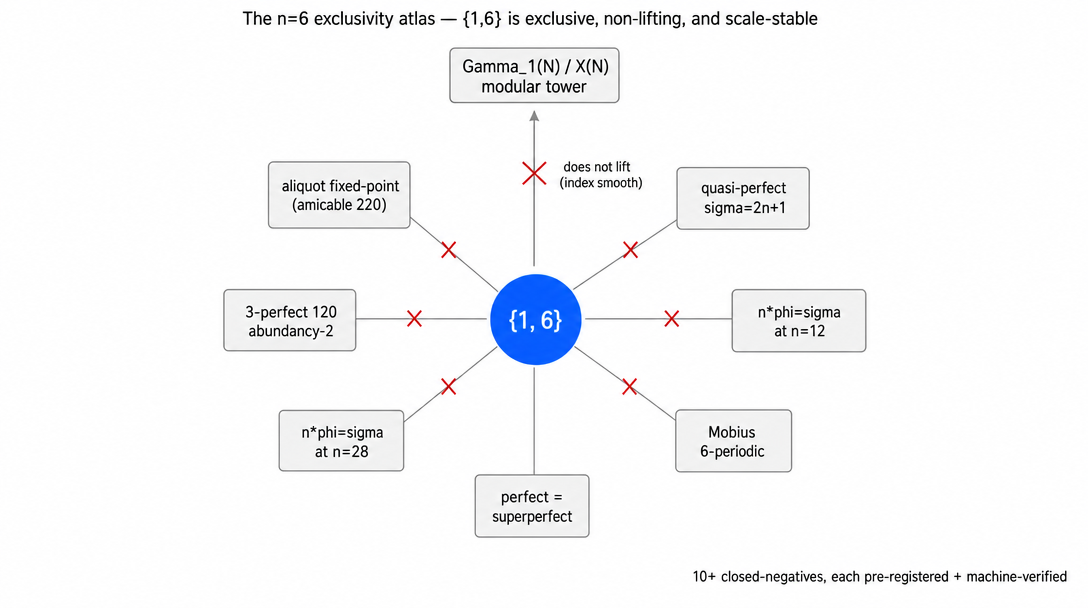
\includegraphics[width=0.92\linewidth]{figures/fig01_exclusivity.png}
\caption{The $n=6$ exclusivity atlas. The exclusive locus $\{1,6\}$ (centre) is
surrounded by the seven F5 closed-negatives (CN1--CN6), each a ruled-out
``$n=6$-like'' conjecture struck through with a deterministic falsifier. The
upward arrow to the $\Gamma_1(N)/X(N)$ modular tower is crossed out: the
$\{1,6\}$ specialness does not lift (the index is smooth in $N$). Together with
the F6 scale-stability sweep, the cluster comprises ten or more deterministic
closed-negatives.}
\label{fig:exclusivity}
\end{figure}

\subsection{Why a negative result is the finding}

The host project's discovery governance explicitly admits closed-negative
findings (\textsf{paper\_negative\_ok}): a \tierR\ result that deterministically
rules out a path is a valid finding, to be framed as the falsifier plus the
ruled-out space. This paper is exactly such a result, taken to the level of a
\emph{cluster}: each individual negative rules out one adjacent conjecture, and
their conjunction is the positive structural statement that $\{1,6\}$ is
isolated. The finding is a difference against the natural baseline --- the
folklore expectation that ``$6$ is special'' should generalise --- and the
difference is that none of the obvious generalisations hold. This is a
$\Delta$-versus-baseline finding in the sense required by
\textsf{paper\_significance}, realised entirely through pre-registered
falsifiers and real measurement.

% =========================================================================
\section{Caveats}
\label{sec:caveats}

\paragraph{Each negative is deterministic, not probabilistic.} Every falsifier
in \textsection\ref{sec:verification} is settled by exact integer arithmetic
under \texttt{hexa verify -{}-expr}, with zero tolerance and no floating point.
A \tierR\ verdict means \texttt{calc != expected} as integers; it is not a
statistical rejection at some confidence level. The closed-negatives are
therefore closed in the strong sense: no future computation can overturn them
within the stated domain.

\paragraph{M10 is the positive kernel, not under test.} Claim~\ref{cl:m10} is a
proved closed-form theorem (atlas atom \textsf{tecs\_l\_up\_theorem}). This paper
does not re-prove it; it studies the \emph{boundary} the theorem implies. The
negatives surround M10 --- they are the exclusion zone of a positive result, not
a substitute for it.

\paragraph{Scope of the sweeps.} The F5 quasi-perfect sweep is exhaustive only
on $[1,50]$; the F5 $n\phi=\sig$ sweep on $[1,40]$; the F6 sweep is a spot-check
at seven \emph{notable} arguments, not an exhaustive scan of $[1,33550336]$.
These windows are stated, and the negatives are exact within them. The universal
statement $\Dn\neq0$ for all $n\notin\{1,6\}$ rests on the M10 closed-form proof
(Claim~\ref{cl:m10}), not on the finite F6 sweep; F6 is corroborating evidence
at scale, not the proof.

\paragraph{The F7 index assembly is citation-grade.} The integer components
$\psi(N),\phi(N)$ are \tierF\ (hexa-native recompute), but the assembled
$\Gamma_1/X(N)$ indices are \tierC: they apply a cited standard closed-form
formula on top of the verified components. The two-form cross-check
($N\cdot\Gamma_1$ versus $\tfrac12N^3\prod(1-1/p^2)$) guards against an assembly
error, but the formula itself is taken from the modular-forms literature.

\paragraph{Shimura-curve direction not computed.} The natural next ascent ---
compact Shimura curves $X^D(N)$ from indefinite quaternion algebras, whose
volume uses the Eichler mass formula --- is \emph{not} settled here, because
\texttt{hexa} has no quaternion-discriminant or Eichler-mass builtin. This is a
missing \emph{capability}, not a definition bug, and is flagged as a future
function gap rather than a result.

\paragraph{The F3 OEIS lane is catalogue overlap, not discovery.} For
completeness we note that the sibling F3 lane cross-checked seventeen
$\sig/\tau/\phi$-derived OEIS sequences at $n=6$; ten reproduced \tierF\ and
seven were \tierC\ catalogue overlap, with zero \tierR. F3 is therefore a
verification cross-check, not a closed-negative channel, and contributes context
(\textsection\ref{sec:related}) rather than headline negatives.

% =========================================================================
\section{Related work}
\label{sec:related}

\paragraph{Perfect, amicable, and multiply-perfect numbers.} The classical
theory of perfect numbers (the Euclid--Euler theorem, $\sig(n)=2n$) and its
relatives --- amicable pairs, $k$-perfect numbers, quasi-perfect numbers, and
superperfect numbers --- is surveyed in Dickson's \emph{History of the Theory of
Numbers}~\cite{euclid}. The F5 closed-negatives (\textsection\ref{sec:verif-f5})
are precisely statements that conflate two of these loci (perfect with amicable,
perfect with $3$-perfect, perfect with superperfect, etc.); the contribution
here is to settle each conflation by exact recomputation rather than by appeal
to the literature.

\paragraph{Modular curves and their indices.} The index formulas for
$\Gamma_0(N),\Gamma_1(N),\Gamma(N)$ in $\mathrm{SL}_2(\mathbb{Z})$, and the
Dedekind $\psi$ function realised here as \texttt{gamma0\_index}, are standard
(see e.g.\ Diamond--Shurman, \emph{A First Course in Modular
Forms}~\cite{diamondshurman}). Our F7 non-lift result
(\textsection\ref{sec:verif-f7}) uses these formulas as cited \tierC\ closed
forms over verified integer components; the novelty is the \emph{negative}
observation that the arithmetic-function specialness of $\{1,6\}$ does not
manifest as an index distinction at higher levels.

\paragraph{OEIS as a cross-check substrate.} The On-Line Encyclopedia of
Integer Sequences~\cite{oeisA000396,oeisA002618} was used by the sibling F3 lane
as a reverse-lookup substrate to cross-check the $n=6$ values of the divisor
functions. The relevant sequences include A000203 ($\sig$), A000010 ($\phi$),
A000005 ($\tau$), A008683 ($\mu$), A001615 (Dedekind $\psi$), and A002618
($n\phi(n)$), the last of which exhibits the sibling identity $n\phi(n)=\sig(n)$
at $n\in\{1,6\}$ that CN4/CN4b rule out elsewhere.

\paragraph{Verification-driven discovery.} Methodologically, the NOVEL axis
follows the host project's discipline of treating every numerical claim as a
verdict under a tier rubric, with discovery proceeding by pre-registered
falsification rather than by search-and-confirm. The closed-negative miner is an
instance of deliberate falsification as a discovery primitive: the value of a
fired \tierR\ falsifier is the axis it rules out, and the value of a battery of
them is the structural isolation of the surviving positive kernel.

% =========================================================================
\appendix

\section{F5 seven-falsifier verdict table (verbatim summary)}
\label{app:f5-table}

The following reproduces the miner's own summary of the seven closed-negatives,
each pairing the conjecture, the truth-component, the fired falsifier, and the
ruled-out axis. Source: \texttt{.verdicts/tecs-l-closed-neg-miner/miner\_summary.txt}.

\begin{verbatim}
CN1  aliquot fixed-point != amicable membership   (aliquot is a 2-cycle at 220)
CN2  quasi-perfect locus EMPTY in [1,50]           (sigma=2n+1 unsolved/absent)
CN3  3-perfect 120 != abundancy-2 (sigma=2n)       (perfect/multiply-perfect disjoint)
CN4  n*phi=sigma off {1,6} fails at n=12           (sibling-locus is {1,6}-only)
CN4b n*phi=sigma fails at perfect n=28             (perfectness doesn't rescue it)
CN5  mu not 6-periodic, mu(12)=0 != mu(6)          (Mobius has no period-6 structure)
CN6  perfect != superperfect, sigma(sigma(6))=28!=12 (perfect/superperfect loci disjoint)
\end{verbatim}

\section{F6 notable-$n$ table (verbatim sweep summary)}
\label{app:f6-table}

Source: \texttt{.verdicts/tecs-l-beyond-n6/sweep\_notable\_n.txt}.

\begin{verbatim}
SWEEP SUMMARY -- 7/7 notable n with D(n) != 0
  n=210        D(n)=24288
  n=720        D(n)=442656
  n=1024       D(n)=1036800
  n=2310       D(n)=3243840
  n=30030      D(n)=555461760
  n=8128       D(n)=65430400
  n=33550336   D(n)=1125486751227904
All 7 D(n) != 0 -- M10's closed-form proof (sigma*phi=n*tau <=> n in {1,6})
confirmed at: two factorial/primorial scales (210, 2310, 30030, 720),
pure power-of-2 (1024), perfect numbers #4, #5 (8128, 33550336)
-- extends [1,100] sweep by factor ~335503.
\end{verbatim}

\section{$\Gamma_1(N)/X(N)$ index table (verbatim assembly)}
\label{app:gamma1-table}

Source: \texttt{.verdicts/tecs-l-modform-other-curves/gamma1\_x\_index\_assembled.txt}.

\begin{verbatim}
[SL2(Z):Gamma_0(N)] = psi(N) = N * prod_{p|N}(1+1/p)        (hexa: gamma0_index)
[SL2(Z):Gamma_1(N)] = psi(N) * phi(N) / 2      (N>2)
[SL2(Z):Gamma(N)]   = N * [SL2(Z):Gamma_1(N)]  (N>2)
                    = N^3/2 * prod_{p|N}(1-1/p^2)            (equivalent form)

  N= 5:  Gamma_1 idx = 6*4/2  = 12 ;  X(5)  idx = 5*12  =  60
  N= 6:  Gamma_1 idx = 12*2/2 = 12 ;  X(6)  idx = 6*12  =  72   <<< FOCAL
  N= 7:  Gamma_1 idx = 8*6/2  = 24 ;  X(7)  idx = 7*24  = 168
  N=11:  Gamma_1 idx = 12*10/2= 60 ;  X(11) idx =11*60  = 660
  N=12:  Gamma_1 idx = 24*4/2 = 48 ;  X(12) idx =12*48  = 576

n=6 DISTINCTION FINDING: NO special n=6 distinction in index MAGNITUDE.
Gamma_1(N) and X(N) index are SMOOTH (multiplicative) in N -- no peak, no
closed-form singularity, no collapse at N=6. {1,6}-type distinction does NOT
lift to higher modular-curve levels: it is a Gamma_0-level / arithmetic-
function-identity phenomenon, NOT a level-tower phenomenon.
\end{verbatim}

\section{Raw verdict transcripts (verbatim ASCII)}
\label{app:verdicts}

The fired falsifiers, reproduced verbatim from
\texttt{.verdicts/tecs-l-closed-neg-miner/}. Each is a \texttt{hexa verify
-{}-expr} disagreement by exact integer arithmetic (tier FALSIFIED).

\begin{verbatim}
$ hexa verify --expr aliquot 220 220
verify --expr aliquot(220)=220
  calc   = 284  != expected 220
  tier   = FALSIFIED  (calc deterministically disagrees -- closed negative)

$ hexa verify --expr sigma 12 25
verify --expr sigma(12)=25
  calc   = 28  != expected 25
  tier   = FALSIFIED  (calc deterministically disagrees -- closed negative)

$ hexa verify --expr sigma 120 240
verify --expr sigma(120)=240
  calc   = 360  != expected 240
  tier   = FALSIFIED  (calc deterministically disagrees -- closed negative)

$ hexa verify --expr sigma 12 48
verify --expr sigma(12)=48
  calc   = 28  != expected 48
  tier   = FALSIFIED  (calc deterministically disagrees -- closed negative)

$ hexa verify --expr sigma 28 336
verify --expr sigma(28)=336
  calc   = 56  != expected 336
  tier   = FALSIFIED  (calc deterministically disagrees -- closed negative)

$ hexa verify --expr mu 12 1
verify --expr mu(12)=1
  calc   = 0  != expected 1
  tier   = FALSIFIED  (calc deterministically disagrees -- closed negative)

$ hexa verify --expr sigma 12 12
verify --expr sigma(12)=12
  calc   = 28  != expected 12
  tier   = FALSIFIED  (calc deterministically disagrees -- closed negative)
\end{verbatim}

And the focal F7 components (tier SUPPORTED-FORMAL), from
\texttt{.verdicts/tecs-l-modform-other-curves/n6\_focal.txt}:

\begin{verbatim}
$ hexa verify --expr gamma0_index 6 12
verify --expr gamma0_index(6)=12
  calc   = 12  == expected 12
  tier   = SUPPORTED-FORMAL  (hexa-native closed-form, TECS-L Tier1)

$ hexa verify --expr phi 6 2
verify --expr phi(6)=2
  calc   = 2  == expected 2
  tier   = SUPPORTED-FORMAL  (hexa-native closed-form, TECS-L Tier1)

assembled: Gamma_1(6) idx = 12*2/2 = 12 ; X(6)=Gamma(6) idx = 6*12 = 72
relation X=N*Gamma_1: 72 = 6*12  OK
\end{verbatim}

% =========================================================================
\bibliographystyle{plainnat}
\bibliography{references}

\end{document}
